
\pgfplotsset{compat=1.17}


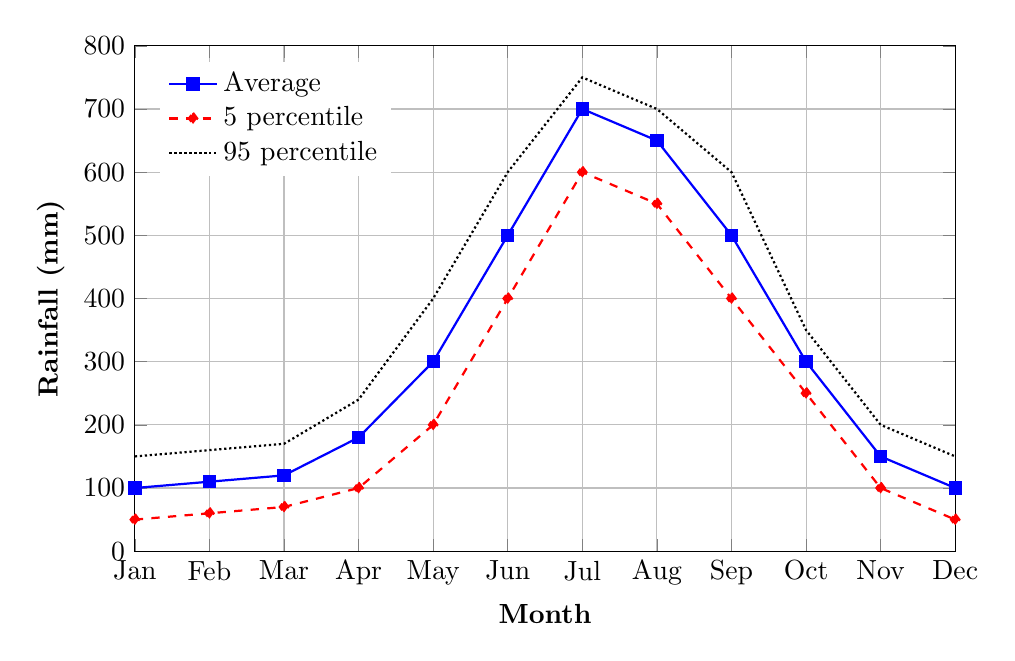
\begin{tikzpicture}
\begin{axis}[
    width=12cm, height=8cm,
    xlabel={\textbf{Month}},
    ylabel={\textbf{Rainfall (mm)}},
    xmin=1, xmax=12,
    ymin=0, ymax=800,
    xtick={1,2,3,4,5,6,7,8,9,10,11,12},
    xticklabels={Jan, Feb, Mar, Apr, May, Jun, Jul, Aug, Sep, Oct, Nov, Dec},
    ytick={0, 100, 200, 300, 400, 500, 600, 700, 800},
    legend pos=north west,
    legend cell align={left},
    legend style={draw=none},
    grid=both
]

% Average Line
\addplot[
    color=blue,
    mark=square*,
    thick
]
coordinates {
    (1,100) (2,110) (3,120) (4,180) (5,300) (6,500) 
    (7,700) (8,650) (9,500) (10,300) (11,150) (12,100)
};
\addlegendentry{Average}

% 5 Percentile Line
\addplot[
    color=red,
    dashed,
    mark=diamond*,
    thick
]
coordinates {
    (1,50) (2,60) (3,70) (4,100) (5,200) (6,400) 
    (7,600) (8,550) (9,400) (10,250) (11,100) (12,50)
};
\addlegendentry{5 percentile}

% 95 Percentile Line
\addplot[
    color=black,
    densely dotted,
    thick
]
coordinates {
    (1,150) (2,160) (3,170) (4,240) (5,400) (6,600) 
    (7,750) (8,700) (9,600) (10,350) (11,200) (12,150)
};
\addlegendentry{95 percentile}

\end{axis}
\end{tikzpicture}
